\documentclass[11pt,a4paper]{article}

\usepackage[T1]{fontenc}
\usepackage[utf8]{inputenc}
\usepackage[french]{babel}
\usepackage{geometry}
\usepackage{enumitem}
\usepackage{amsmath,amssymb}
\usepackage{graphicx}
\usepackage{float}
\usepackage{booktabs}
\usepackage{xcolor}
\usepackage{hyperref}
\usepackage{listings}

\geometry{margin=2.5cm}

\hypersetup{
    colorlinks=true,
    linkcolor=blue,
    urlcolor=blue
}

\lstset{
    basicstyle=\ttfamily\small,
    breaklines=true,
    frame=single,
    columns=fullflexible
}

\title{Projet --- Analyse de la Polarisation}
\author{Nom 1 \and Nom 2 \and Nom 3}
\date{\today}

\begin{document}

\maketitle

\tableofcontents
\newpage

\section{Introduction}

Dans ce projet, nous \'etudions plusieurs mani\`eres de mesurer la polarisation d'un profil \'electoral. L'id\'ee g\'en\'erale est de comparer des profils peu polaris\'es, o\`u les votantes restent proches d'un m\^eme centre, \`a des profils fortement polaris\'es, o\`u l'\'electorat se s\'epare en deux blocs oppos\'es.

Le sujet consid\`ere deux cadres :
\begin{itemize}[leftmargin=*]
    \item les votes par approbation ;
    \item les votes par ordres totaux.
\end{itemize}

Notre travail a consist\'e \`a :
\begin{itemize}[leftmargin=*]
    \item g\'en\'erer des profils al\'eatoires avec un niveau de polarisation contr\^olable ;
    \item impl\'ementer plusieurs mesures de polarisation ;
    \item analyser certaines propri\'et\'es axiomatiques ;
    \item produire des exp\'eriences pour visualiser l'\'evolution de ces mesures.
\end{itemize}

Dans toute la suite, on note \(n\) le nombre de votantes et \(m\) le nombre de candidates.

\section{Description g\'en\'erale de l'impl\'ementation}

Le code du projet est organis\'e autour des modules suivants :
\begin{itemize}[leftmargin=*]
    \item \texttt{src/generation.py} : g\'en\'eration des profils ;
    \item \texttt{src/distances.py} : distances de Hamming et de Spearman ;
    \item \texttt{src/pairwise.py} : quantit\'es \(d^{c_k,c_l}(p)\) ;
    \item \texttt{src/phi2.py} : calcul de \(\phi_2\) ;
    \item \texttt{src/consensus.py} : calcul du consensus global \(u_1\) ;
    \item \texttt{src/clustering.py} : approximation \`a deux groupes \(\widetilde{u_2}\) ;
    \item \texttt{src/measures.py} : calcul de \(\phi_{d_H}\) et \(\phi_{d_S}\) ;
    \item \texttt{src/experiments.py} et \texttt{src/plots.py} : exp\'eriences et graphiques.
\end{itemize}

Toutes les exp\'eriences finales ont \'et\'e g\'en\'er\'ees avec le pipeline :
\begin{lstlisting}
python -m scripts.run_final_pipeline
\end{lstlisting}

\section{Question 1 --- G\'en\'eration al\'eatoire de profils d'approbation}

Pour les votes par approbation, nous avons retenu une g\'en\'eration \`a partir :
\begin{itemize}[leftmargin=*]
    \item d'un bulletin central \(a\) ;
    \item de son bulletin oppos\'e \(\overline{a}\) ;
    \item d'un param\`etre \(\alpha \in [0,1]\) qui contr\^ole le niveau de polarisation ;
    \item d'un param\`etre de bruit \texttt{noise}.
\end{itemize}

Le principe est le suivant :
\begin{itemize}[leftmargin=*]
    \item si \(\alpha\) est proche de \(0\), la majorit\'e des votantes restent proches d'un m\^eme centre ;
    \item si \(\alpha\) est proche de \(1\), le profil se rapproche d'une r\'epartition en deux blocs oppos\'es ;
    \item le bruit permet d'\'eviter d'obtenir des profils trop artificiels.
\end{itemize}

Cette m\'ethode est impl\'ement\'ee dans \texttt{generate\_approval\_profile(n, m, alpha, noise, seed)}.

\paragraph{Justification du choix}
Ce sch\'ema a l'avantage d'\^etre simple \`a param\'etrer, facile \`a expliquer, et surtout compatible avec l'intuition demand\'ee dans le sujet : faible polarisation autour d'un centre unique, forte polarisation autour de deux p\^oles oppos\'es.

\paragraph{Exemple}
Si \(m=4\) et que le centre vaut \(a=(1,0,1,0)\), alors :
\begin{itemize}[leftmargin=*]
    \item pour une faible polarisation, on peut obtenir un profil du type
    \[
    (1,0,1,0),\ (1,0,1,0),\ (1,0,0,0),\ (1,0,1,1),
    \]
    c'est-\`a-dire des bulletins proches du centre ;
    \item pour une forte polarisation, on peut au contraire obtenir un profil de la forme
    \[
    (1,0,1,0),\ (1,0,1,0),\ (0,1,0,1),\ (0,1,0,1),
    \]
    qui se rapproche de deux blocs oppos\'es.
\end{itemize}

\section{Question 2 --- G\'en\'eration al\'eatoire de profils par ordres totaux}

Pour les votes par ordres totaux, nous avons utilis\'e une m\'ethode analogue :
\begin{itemize}[leftmargin=*]
    \item on tire un ordre central \(\sigma\) ;
    \item on consid\`ere son ordre inverse comme p\^ole oppos\'e ;
    \item le param\`etre \(\alpha\) d\'etermine la proportion de votantes proches de chaque p\^ole ;
    \item un bruit est ajout\'e sous la forme d'un nombre contr\^ol\'e d'\'echanges al\'eatoires dans le classement.
\end{itemize}

Cette m\'ethode est impl\'ement\'ee dans \texttt{generate\_ranking\_profile(n, m, alpha, noise, seed)}.

\paragraph{Justification du choix}
Le recours \`a l'ordre inverse comme second p\^ole est naturel, car il fournit une opposition forte et simple \`a interpr\'eter. Le bruit par \'echanges permet d'obtenir des profils plus r\'ealistes sans casser la logique globale de polarisation.

\paragraph{Exemple}
Si \(m=4\) et que l'ordre central est \((c_1,c_2,c_3,c_4)\), alors :
\begin{itemize}[leftmargin=*]
    \item pour une faible polarisation, un profil typique ressemble \`a
    \[
    (c_1,c_2,c_3,c_4),\ (c_1,c_3,c_2,c_4),\ (c_1,c_2,c_4,c_3),
    \]
    o\`u les classements restent proches les uns des autres ;
    \item pour une forte polarisation, on se rapproche plut\^ot de deux blocs oppos\'es, par exemple
    \[
    (c_1,c_2,c_3,c_4),\ (c_1,c_2,c_3,c_4),\ (c_4,c_3,c_2,c_1),\ (c_4,c_3,c_2,c_1).
    \]
\end{itemize}

\section{Question 4 --- Quels axiomes sont satisfaits par \texorpdfstring{$\phi_2$}{phi2} ?}

Nous rappelons que le sujet d\'efinit :
\[
\phi_2(p)=\sum_{\{c_k,c_l\}\in C^2}\frac{n-d^{c_k,c_l}(p)}{n\binom{m}{2}},
\]
avec
\[
d^{c_k,c_l}(p)=|n_{c_kc_l}(p)-n_{c_lc_k}(p)|.
\]

\subsection*{Discussion g\'en\'erale}

Notre impl\'ementation suit cette d\'efinition dans \texttt{src/pairwise.py} et \texttt{src/phi2.py}. Les exp\'eriences montrent que la mesure cro\^\i t globalement lorsque le niveau de polarisation augmente.

\subsection*{R\'egularit\'e}

On a toujours \(0 \le d^{c_k,c_l}(p) \le n\), donc
\[
0 \le \frac{n-d^{c_k,c_l}(p)}{n\binom{m}{2}} \le \frac{1}{\binom{m}{2}}.
\]
En sommant sur toutes les paires, on obtient bien
\[
0 \le \phi_2(p) \le 1.
\]

En revanche, la partie forte de l'axiome de r\'egularit\'e n'est pas satisfaite dans toute sa forme.

\paragraph{Pourquoi \(\phi_2(p)=0\) n'est pas \'equivalent \`a un profil de la forme \(p_a\) dans le cas approval}
Consid\'erons le profil homog\`ene o\`u toutes les votantes ont le bulletin \((1,1)\). Pour l'unique paire \(\{c_1,c_2\}\), on a
\[
n_{c_1c_2}(p)=0,\qquad n_{c_2c_1}(p)=0,
\]
donc \(d^{c_1,c_2}(p)=0\), et ainsi \(\phi_2(p)=1\). Pourtant, le profil est parfaitement homog\`ene. La caract\'erisation \(\phi_2(p)=0 \Leftrightarrow p=p_a\) n'est donc pas vraie en g\'en\'eral dans le cadre approval.

\paragraph{Pourquoi \(\phi_2(p)=1\) n'est pas forc\'ement \'equivalent \`a un profil exactement bipolaire}
Dans le cas ranking, on peut construire des profils o\`u chaque paire de candidates est partag\'ee \'equitablement sans que le profil soit exactement de la forme \(p_{\sigma,\bar{\sigma}}\). La valeur \(1\) traduit donc surtout un \'equilibre parfait au niveau paire \`a paire, pas n\'ecessairement une structure strictement bipolaire unique.

Ainsi, \(\phi_2\) v\'erifie bien la borne \([0,1]\), mais pas la caract\'erisation forte demand\'ee par l'axiome 1.

\subsection*{Neutralit\'e}

La mesure est neutre. En effet, si l'on permute les candidates par une permutation \(\pi\), chaque paire \(\{c_k,c_l\}\) est simplement renomm\'ee en \(\{\pi(c_k),\pi(c_l)\}\). Les nombres \(n_{c_kc_l}(p)\) et \(n_{c_lc_k}(p)\) sont donc eux aussi seulement renomm\'es, sans changer leurs valeurs. L'ensemble des termes de la somme d\'efinissant \(\phi_2\) reste inchang\'e. Par cons\'equent,
\[
\phi_2(p)=\phi_2(p^\pi).
\]

\subsection*{Anonymat}

La mesure est anonyme. En effet, permuter les votantes ne change pas le nombre de votantes qui pr\'ef\`erent \(c_k\) \`a \(c_l\), ni celui des votantes qui pr\'ef\`erent \(c_l\) \`a \(c_k\). Les quantit\'es \(n_{c_kc_l}(p)\), \(d^{c_k,c_l}(p)\) et donc \(\phi_2(p)\) restent inchang\'ees. Ainsi,
\[
\phi_2(p)=\phi_2(fp)
\]
pour toute permutation \(f\) des votantes.

\subsection*{Invariance par r\'eplication}

La mesure est invariante par r\'eplication. Si l'on remplace le profil \(p\) par \(kp\), alors tous les effectifs \(n_{c_kc_l}(p)\) sont multipli\'es par \(k\). On a donc
\[
n_{c_kc_l}(kp)=k\,n_{c_kc_l}(p), \qquad d^{c_k,c_l}(kp)=k\,d^{c_k,c_l}(p),
\]
et le nombre total de votantes devient \(kn\). Pour chaque paire,
\[
\frac{kn-kd^{c_k,c_l}(p)}{kn\binom{m}{2}}=\frac{n-d^{c_k,c_l}(p)}{n\binom{m}{2}}.
\]
La somme totale est donc inchang\'ee, ce qui donne
\[
\phi_2(kp)=\phi_2(p).
\]

\paragraph{Conclusion pour la question 4}
La mesure \(\phi_2\) v\'erifie :
\begin{itemize}[leftmargin=*]
    \item la borne \(0 \le \phi_2 \le 1\) ;
    \item la neutralit\'e ;
    \item l'anonymat ;
    \item l'invariance par r\'eplication.
\end{itemize}
En revanche, la version forte de la r\'egularit\'e, avec caract\'erisation exacte des cas \(\phi_2=0\) et \(\phi_2=1\), n'est pas satisfaite en g\'en\'eral.

\section{Question 6 --- Exp\'eriences sur \texorpdfstring{$\phi_2$}{phi2}}

Pour cette question, nous avons fait varier le param\`etre de polarisation \(\alpha\) entre \(0\) et \(1\) par pas de \(0.1\), avec :
\begin{itemize}[leftmargin=*]
    \item \(n = 40\) votantes ;
    \item \(m = 6\) candidates ;
    \item \(20\) essais par valeur de \(\alpha\) pour \(\phi_2\).
\end{itemize}

\subsection{Cas approval}

\begin{figure}[H]
    \centering
    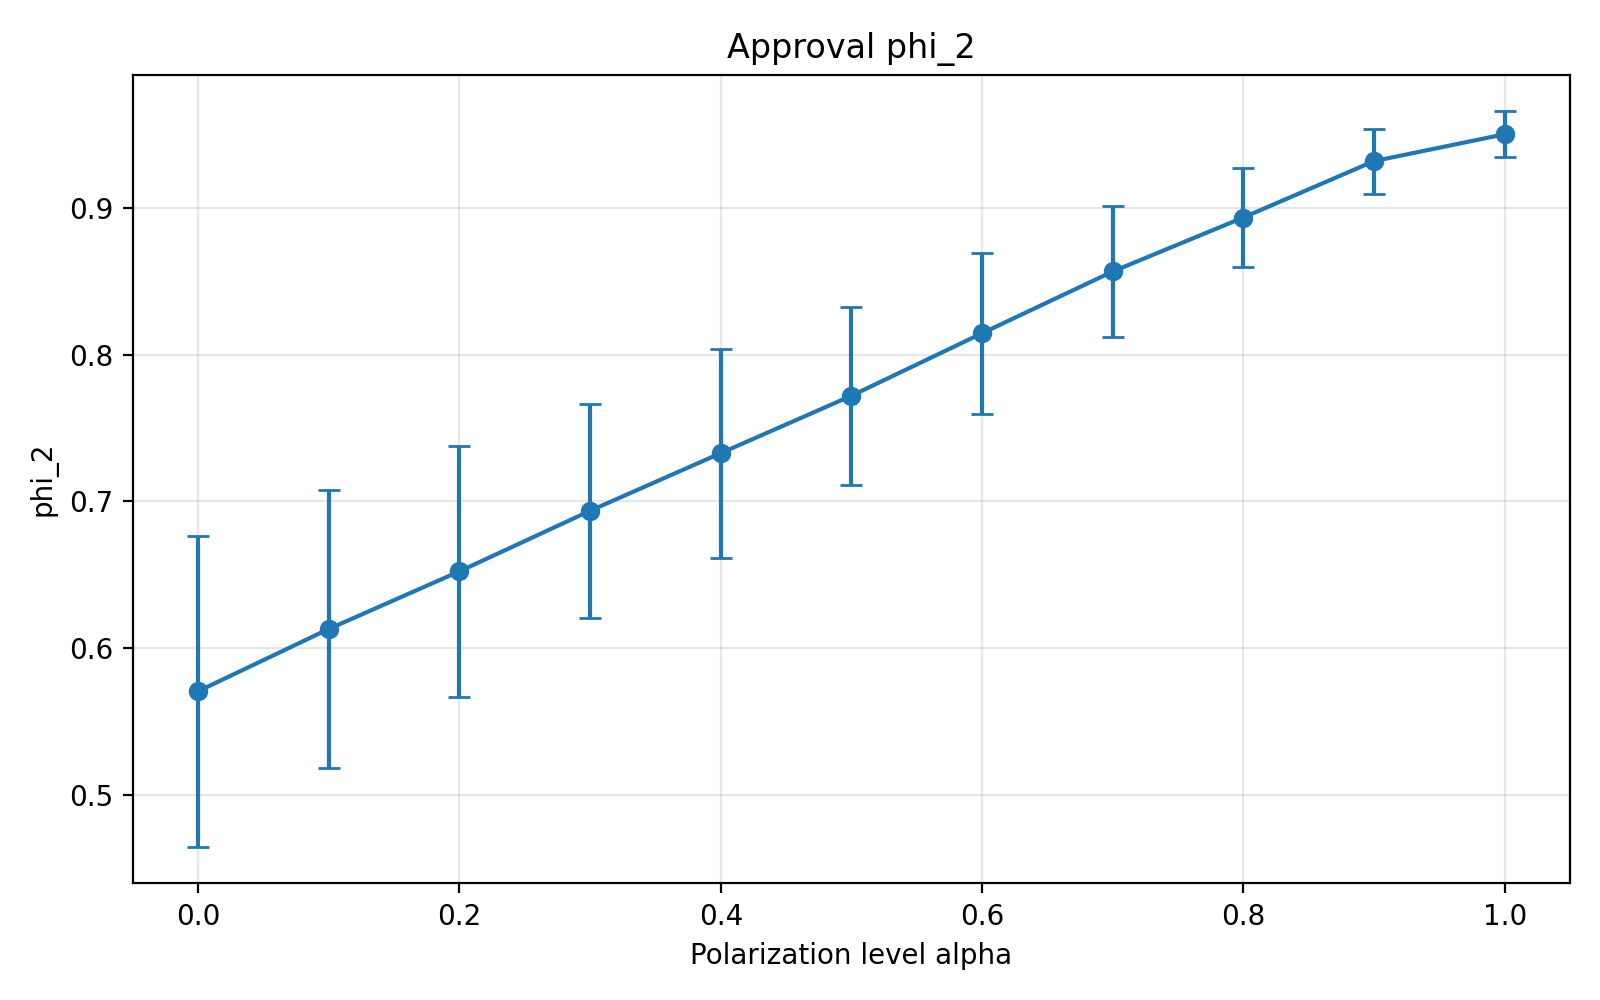
\includegraphics[width=0.82\textwidth]{../outputs/figures/final_phi2_approval.png}
    \caption{\'Evolution de \(\phi_2\) pour les profils approval.}
\end{figure}

On observe une augmentation nette de la mesure lorsque \(\alpha\) augmente. La moyenne passe d'environ \(0.571\) pour \(\alpha=0\) \`a environ \(0.951\) pour \(\alpha=1\). Cela est coh\'erent avec l'id\'ee que la mesure d\'etecte correctement le passage d'un profil peu polaris\'e \`a un profil fortement bipolaire.

\subsection{Cas ranking}

\begin{figure}[H]
    \centering
    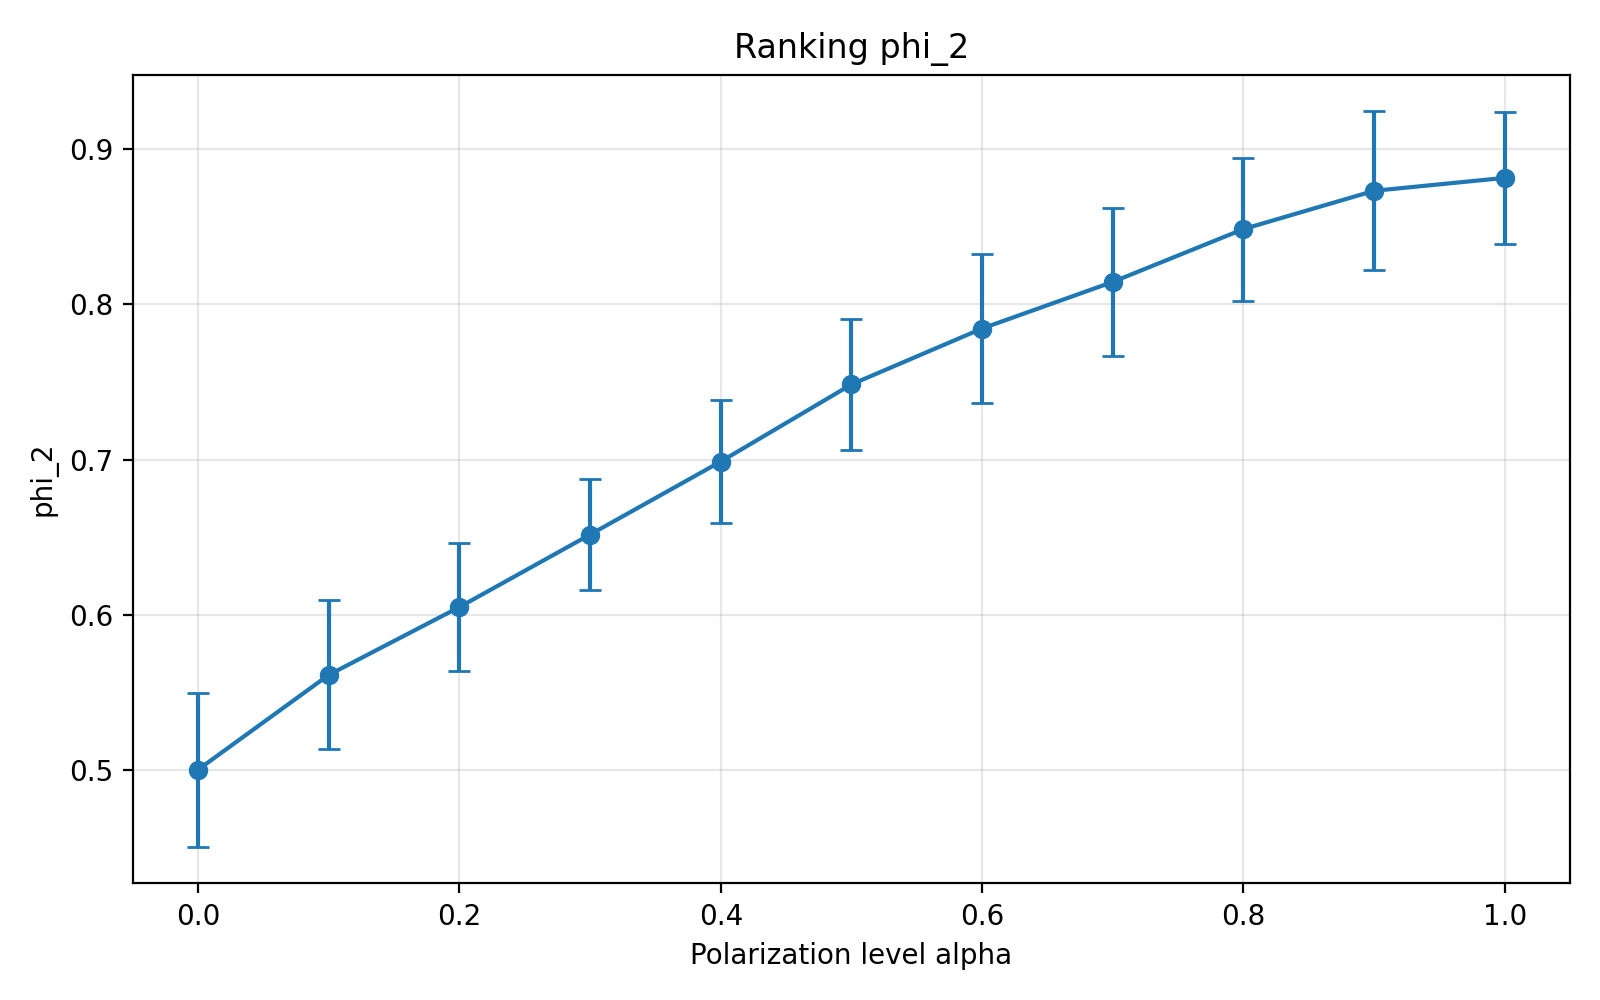
\includegraphics[width=0.82\textwidth]{../outputs/figures/final_phi2_ranking.png}
    \caption{\'Evolution de \(\phi_2\) pour les profils ranking.}
\end{figure}

Le comportement est similaire : la moyenne augmente d'environ \(0.500\) \`a \(0.881\). La croissance est r\'eguli\`ere et confirme que la g\'en\'eration retenue pour les profils ranking produit bien des instances de plus en plus polaris\'ees lorsque \(\alpha\) cro\^\i t.

\paragraph{Conclusion exp\'erimentale}
Dans les deux cadres, \(\phi_2\) r\'eagit dans le sens attendu au param\`etre de polarisation. Cela valide \`a la fois la m\'ethode de g\'en\'eration et l'impl\'ementation de la mesure.

\section{Question 7 --- Montrer que \texorpdfstring{$d_H$}{dH} et \texorpdfstring{$d_S$}{dS} sont des distances}

Les deux distances utilis\'ees dans le projet sont :
\begin{itemize}[leftmargin=*]
    \item la distance de Hamming sur les votes par approbation ;
    \item la distance de Spearman sur les ordres totaux.
\end{itemize}

\subsection*{Plan de r\'edaction conseill\'e}

\paragraph{Pour \(d_H\)}
Soient \(a,b,c \in \{0,1\}^m\).
\begin{itemize}[leftmargin=*]
    \item \emph{Positivit\'e} : chaque terme \(1_{a[i]\ne b[i]}\) vaut \(0\) ou \(1\), donc
    \[
    d_H(a,b)=\sum_{i=1}^m 1_{a[i]\ne b[i]} \ge 0.
    \]
    \item \emph{S\'eparation} : \(d_H(a,b)=0\) si et seulement si aucun indice ne diff\`ere, donc si et seulement si \(a=b\).
    \item \emph{Sym\'etrie} : la condition \(a[i]\ne b[i]\) est \'equivalente \`a \(b[i]\ne a[i]\), donc
    \[
    d_H(a,b)=d_H(b,a).
    \]
    \item \emph{In\'egalit\'e triangulaire} : si \(a[i]\ne c[i]\), alors au moins l'un des deux \'ev\'enements \(a[i]\ne b[i]\) ou \(b[i]\ne c[i]\) est vrai. Ainsi,
    \[
    1_{a[i]\ne c[i]} \le 1_{a[i]\ne b[i]} + 1_{b[i]\ne c[i]}.
    \]
    En sommant sur tous les indices \(i\), on obtient
    \[
    d_H(a,c)\le d_H(a,b)+d_H(b,c).
    \]
\end{itemize}
Ainsi, \(d_H\) est bien une distance.

\paragraph{Pour \(d_S\)}
Soient \(\sigma,\tau,\rho\) trois ordres totaux sur \(C\), et \(r_\sigma, r_\tau, r_\rho\) les fonctions de rang associ\'ees.
\begin{itemize}[leftmargin=*]
    \item \emph{Positivit\'e} :
    \[
    d_S(\sigma,\tau)=\sum_{c\in C}|r_\sigma(c)-r_\tau(c)| \ge 0.
    \]
    \item \emph{S\'eparation} : si \(d_S(\sigma,\tau)=0\), alors pour toute candidate \(c\),
    \[
    |r_\sigma(c)-r_\tau(c)|=0,
    \]
    donc \(r_\sigma(c)=r_\tau(c)\). Les deux ordres sont donc identiques.
    \item \emph{Sym\'etrie} : pour toute candidate \(c\),
    \[
    |r_\sigma(c)-r_\tau(c)| = |r_\tau(c)-r_\sigma(c)|,
    \]
    donc \(d_S(\sigma,\tau)=d_S(\tau,\sigma)\).
    \item \emph{In\'egalit\'e triangulaire} : pour chaque candidate \(c\), l'in\'egalit\'e triangulaire sur \(\mathbb{R}\) donne
    \[
    |r_\sigma(c)-r_\rho(c)| \le |r_\sigma(c)-r_\tau(c)| + |r_\tau(c)-r_\rho(c)|.
    \]
    En sommant sur toutes les candidates,
    \[
    d_S(\sigma,\rho)\le d_S(\sigma,\tau)+d_S(\tau,\rho).
    \]
\end{itemize}
Ainsi, \(d_S\) est bien une distance.

\paragraph{Appui algorithmique}
Ces deux fonctions sont impl\'ement\'ees dans \texttt{src/distances.py} sous les noms :
\begin{itemize}[leftmargin=*]
    \item \texttt{hamming\_distance(a, b)}
    \item \texttt{spearman\_distance(order1, order2)}
\end{itemize}

Le code ne remplace pas les preuves, mais il a permis de valider des cas tests simples.

\section{Question 9 --- Quels axiomes sont satisfaits par \texorpdfstring{$\phi_{d_H}$}{phi dH} et \texorpdfstring{$\phi_{d_S}$}{phi dS} ?}

Les mesures utilis\'ees sont :
\[
\phi_{d_H}(p)=\frac{2}{nm}\bigl(u_1(p)-\widetilde{u_2}(p)\bigr)
\]
et
\[
\phi_{d_S}(p)=\frac{4}{nm^2}\bigl(u_1(p)-\widetilde{u_2}(p)\bigr).
\]

\subsection*{Commentaires}

Ces mesures comparent :
\begin{itemize}[leftmargin=*]
    \item le co\^ut d'un consensus global unique ;
    \item le co\^ut d'une partition en deux groupes avec deux centro\"\i des.
\end{itemize}

Intuitivement, plus l'\'electorat se s\'epare en deux blocs, plus le gain apport\'e par deux centro\"\i des devient important.

\subsection*{Neutralit\'e}

Si l'on raisonne sur la version id\'eale de la mesure, o\`u \(u_2\) est la vraie valeur optimale du probl\`eme \`a deux centro\"\i des, alors la neutralit\'e est v\'erifi\'ee. Une permutation des candidates ne change pas les distances entre bulletins : elle ne fait que renommer les candidates. Les valeurs \(u_1\) et \(u_2\) sont donc inchang\'ees, et la mesure aussi.

\subsection*{Anonymat}

La mesure est anonyme. En effet, \(u_1\) et \(u_2\) ne d\'ependent que de l'ensemble des bulletins pr\'esents, pas de l'ordre dans lequel ils sont list\'es. Une permutation des votantes ne change donc ni \(u_1\), ni \(u_2\), ni la valeur finale de la mesure.

\subsection*{Invariance par r\'eplication}

Si l'on remplace \(p\) par \(kp\), alors tous les co\^uts de distance sont multipli\'es par \(k\) :
\[
u_1(kp)=k\,u_1(p), \qquad u_2(kp)=k\,u_2(p).
\]
Le facteur \(k\) est alors compens\'e par le nouveau nombre de votantes \(kn\) dans le facteur de normalisation. On obtient donc
\[
\phi_{d_H}(kp)=\phi_{d_H}(p)
\]
et de m\^eme pour \(\phi_{d_S}\).

\subsection*{R\'egularit\'e}

On a toujours \(u_2(p)\le u_1(p)\), donc les mesures sont toujours positives ou nulles. De plus, dans les profils unanimistes, on a \(u_1=u_2=0\), donc la mesure vaut \(0\).

Pour les profils parfaitement bipolaires, le consensus \`a deux centro\"\i des devient beaucoup plus performant que le consensus global, et la mesure devient grande. Dans le cas approval, le profil \(p_{a,\bar a}\) donne bien la valeur \(1\) pour la version id\'eale de \(\phi_{d_H}\).

En revanche, la caract\'erisation exacte de tous les cas d'\'egalit\'e \`a \(1\) est plus d\'elicate, en particulier dans le cas ranking. En pratique, nos exp\'eriences montrent que la mesure reste bien dans \([0,1]\), mais la preuve g\'en\'erale compl\`ete des cas extr\^emes demanderait une \'etude plus pouss\'ee.

\paragraph{Conclusion pour la question 9}
Les mesures bas\'ees sur les distances v\'erifient clairement :
\begin{itemize}[leftmargin=*]
    \item l'anonymat ;
    \item la neutralit\'e ;
    \item l'invariance par r\'eplication ;
    \item la nullit\'e sur les profils unanimistes.
\end{itemize}
La discussion des cas extr\^emes de r\'egularit\'e est plus simple dans le cadre approval que dans le cadre ranking.

\section{Question 10 --- Calcul efficace de \texorpdfstring{$u_1$}{u1} pour les votes par approbation}

Dans le cas des votes par approbation, le probl\`eme consiste \`a trouver un bulletin \(a \in \{0,1\}^m\) qui minimise
\[
\sum_{a' \in p} d_H(a,a').
\]

\subsection*{Id\'ee}

La distance de Hamming se s\'eparant coordonn\'ee par coordonn\'ee, il suffit de traiter chaque candidate ind\'ependamment :
\begin{itemize}[leftmargin=*]
    \item si une majorit\'e de votantes approuvent la candidate, le consensus met \(1\) ;
    \item sinon, le consensus met \(0\).
\end{itemize}

Ainsi, le bulletin de consensus est obtenu par vote majoritaire sur chaque composante.

\subsection*{Impl\'ementation}

Cette id\'ee est impl\'ement\'ee dans :
\begin{itemize}[leftmargin=*]
    \item \texttt{approval\_consensus\_ballot(profile)}
    \item \texttt{u1\_approval(profile)}
\end{itemize}

\paragraph{Conclusion}
Le calcul est efficace car il se ram\`ene \`a compter, pour chaque position, le nombre de \(1\) et de \(0\).

\section{Question 11 --- Calcul efficace de \texorpdfstring{$u_1$}{u1} pour les ordres totaux}

Dans le cas des ordres totaux, on cherche un ordre de consensus minimisant la somme des distances de Spearman \`a tous les votes du profil.

\subsection*{Id\'ee de mod\'elisation}

On peut voir ce probl\`eme comme une affectation des candidates aux positions finales du classement. Pour chaque candidate \(c\) et chaque position \(r\), on calcule le co\^ut :
\[
\sum_{v \in V} |r_v(c)-r|.
\]

On obtient ainsi une matrice de co\^uts \emph{candidate $\times$ position}. Le probl\`eme revient ensuite \`a choisir une affectation bijective minimisant la somme totale, ce qui correspond \`a un probl\`eme de couplage parfait de poids minimum dans un graphe biparti.

\subsection*{Impl\'ementation retenue}

Dans notre code, cette id\'ee est impl\'ement\'ee par programmation dynamique sur les sous-ensembles :
\begin{itemize}[leftmargin=*]
    \item \texttt{ranking\_assignment\_costs(profile)} construit la matrice de co\^uts ;
    \item \texttt{ranking\_consensus\_ballot(profile)} cherche l'affectation optimale ;
    \item \texttt{u1\_ranking(profile)} calcule ensuite le co\^ut total du consensus obtenu.
\end{itemize}

\paragraph{Remarque}
Cette solution est exacte et suffit pour les tailles de \(m\) utilis\'ees dans nos exp\'eriences. Elle suit bien l'esprit de l'indication du sujet, m\^eme si l'on n'utilise pas directement \texttt{scipy}.

\paragraph{Complexit\'e}
Si \(m\) est le nombre de candidates, la programmation dynamique explore les sous-ensembles de candidates d\'ej\`a plac\'ees. Le nombre d'\'etats est donc de l'ordre de \(m2^m\), ce qui reste raisonnable pour les valeurs modestes de \(m\) utilis\'ees dans nos exp\'eriences, mais ne serait pas adapt\'e \`a des instances tr\`es grandes.

\section{Question 15 --- Exp\'eriences sur \texorpdfstring{$\phi_{d_H}$}{phi dH} et \texorpdfstring{$\phi_{d_S}$}{phi dS}}

Pour cette question, nous avons utilis\'e le m\^eme protocole global sur \(\alpha \in \{0, 0.1, \dots, 1\}\), avec :
\begin{itemize}[leftmargin=*]
    \item \(n = 40\),
    \item \(m = 6\),
    \item \(10\) essais par valeur de \(\alpha\),
    \item \(10\) relances pour l'algorithme de clustering \`a deux groupes.
\end{itemize}

\subsection{Cas approval : \texorpdfstring{$\phi_{d_H}$}{phi dH}}

\begin{figure}[H]
    \centering
    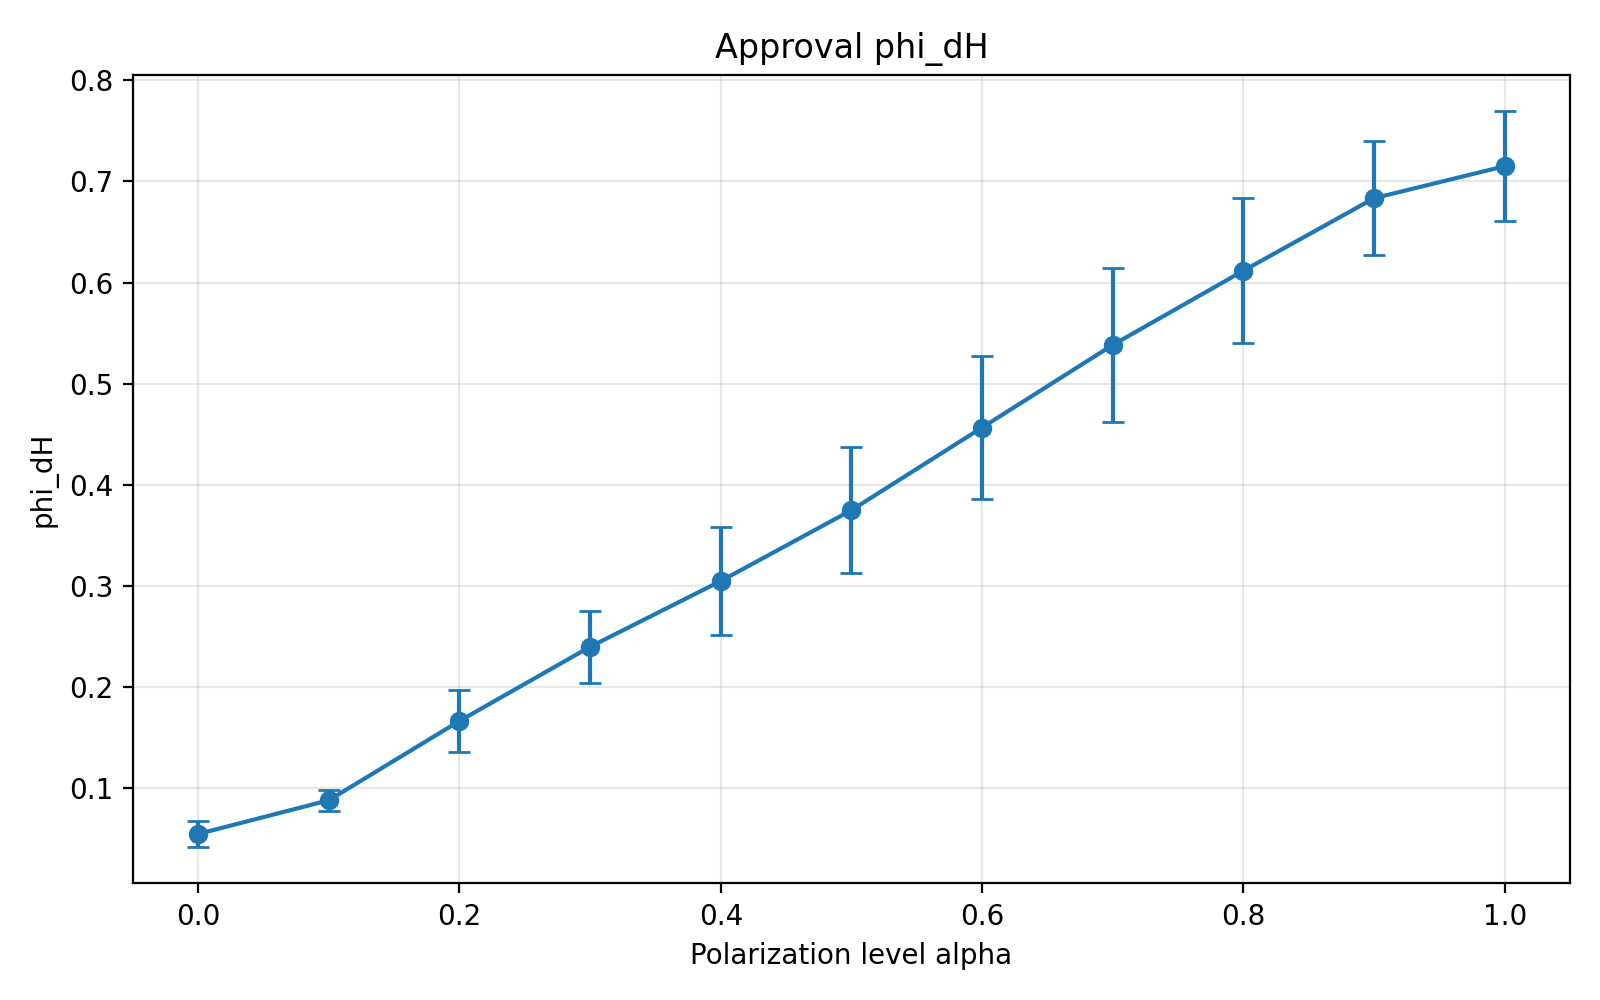
\includegraphics[width=0.82\textwidth]{../outputs/figures/final_phidh_approval.png}
    \caption{\'Evolution de \(\phi_{d_H}\) pour les profils approval.}
\end{figure}

La courbe est fortement croissante. La moyenne passe d'environ \(0.055\) \`a \(0.715\), ce qui montre que plus le profil est polaris\'e, plus un consensus \`a deux blocs devient meilleur qu'un consensus global unique.

\subsection{Cas ranking : \texorpdfstring{$\phi_{d_S}$}{phi dS}}

\begin{figure}[H]
    \centering
    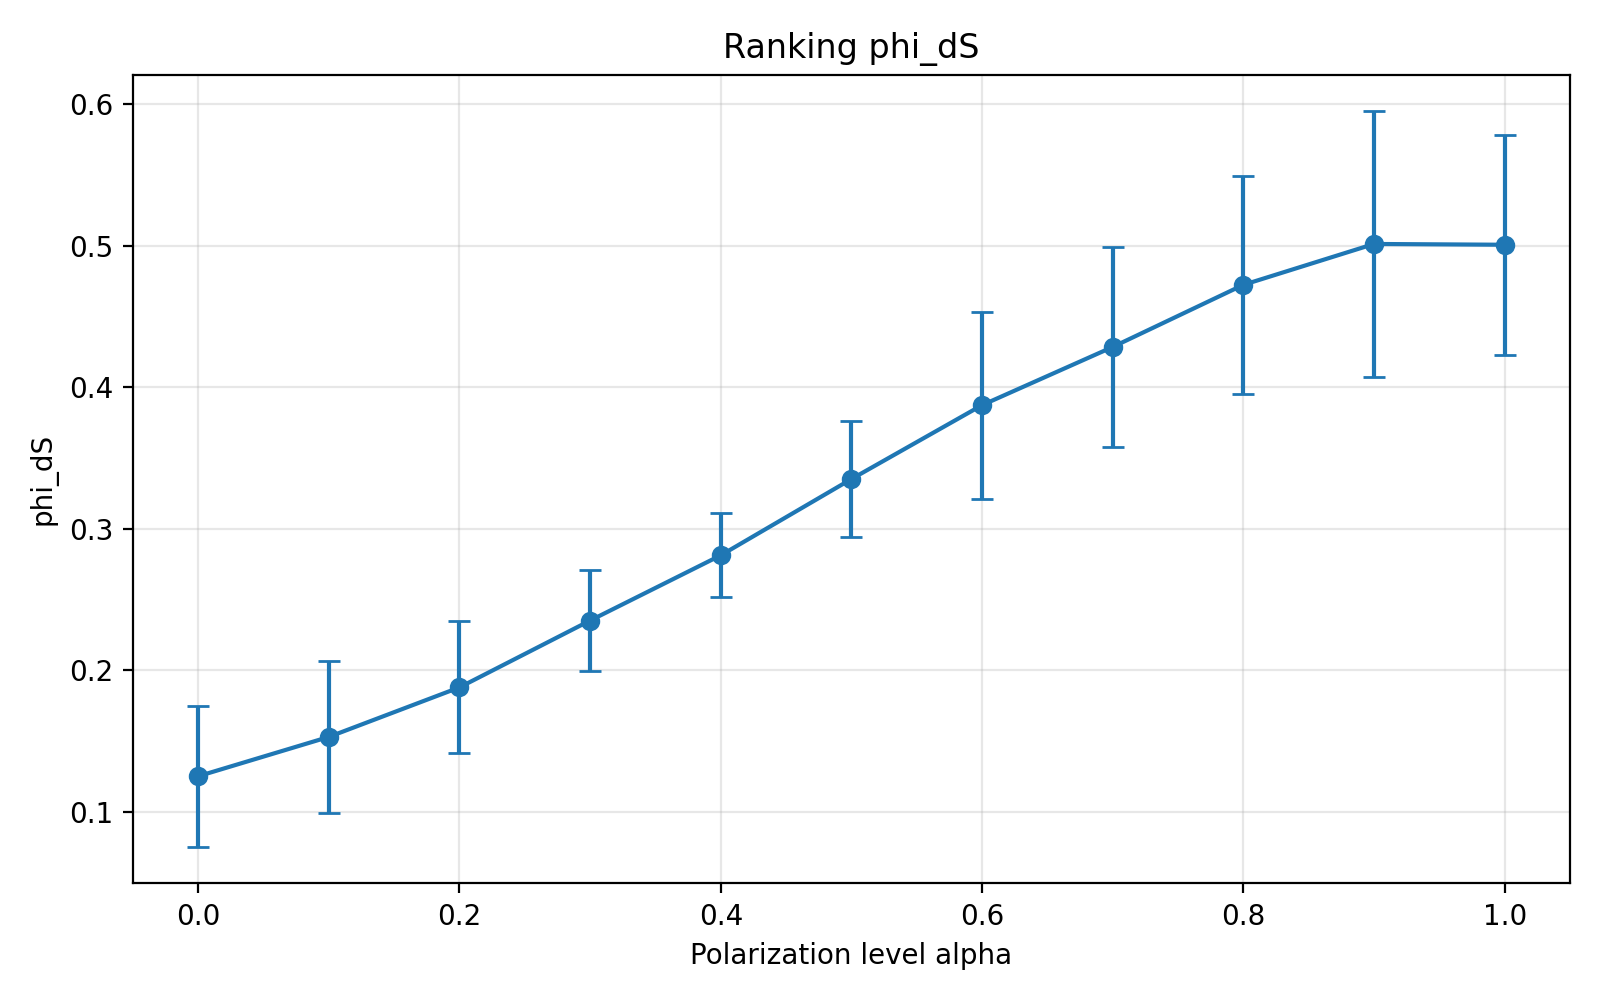
\includegraphics[width=0.82\textwidth]{../outputs/figures/final_phids_ranking.png}
    \caption{\'Evolution de \(\phi_{d_S}\) pour les profils ranking.}
\end{figure}

La moyenne passe d'environ \(0.125\) \`a \(0.501\). La tendance est globalement croissante. La partie finale de la courbe reste un peu plus bruit\'ee que dans le cas approval, mais le signal reste coh\'erent avec l'intuition de polarisation.

\paragraph{Interpr\'etation}
Ces r\'esultats montrent que les mesures bas\'ees sur les distances d\'etectent elles aussi l'augmentation du niveau de polarisation. Elles compl\`etent utilement \(\phi_2\), qui repose davantage sur l'analyse paire \`a paire des pr\'ef\'erences.

\section{Utilisation des IA g\'en\'eratives}

Nous avons utilis\'e des IA g\'en\'eratives principalement comme outils d'assistance technique et r\'edactionnelle. Les usages principaux ont \'et\'e :
\begin{itemize}[leftmargin=*]
    \item proposer une structure de projet en Python ;
    \item g\'en\'erer une premi\`ere version de certaines fonctions ;
    \item ajouter des commentaires de code ;
    \item aider \`a structurer les rapports interm\'ediaires et le rapport final ;
    \item aider au d\'ebogage de l'environnement et \`a l'automatisation des exp\'eriences.
\end{itemize}

Le nombre exact de prompts n'a pas \'et\'e compt\'e \`a l'unit\'e, mais il s'agit d'un usage r\'egulier tout au long du projet, avec plusieurs dizaines d'interactions courtes ou moyennes.

\paragraph{Apports utiles}
\begin{itemize}[leftmargin=*]
    \item L'IA a permis d'acc\'el\'erer fortement la mise en place du squelette du projet.
    \item Elle a \'et\'e utile pour organiser le code, proposer des interfaces de fonctions et r\'ediger des commentaires.
    \item Elle a aussi permis de gagner du temps sur les scripts exp\'erimentaux et sur la structuration des rapports interm\'ediaires.
\end{itemize}

\paragraph{Limites observ\'ees}
\begin{itemize}[leftmargin=*]
    \item Certaines propositions initiales n'\'etaient pas exactement align\'ees avec le PDF.
    \item En particulier, la premi\`ere version de \(\phi_2\) et de \(d^{c_k,c_l}(p)\) a d\^u \^etre corrig\'ee manuellement apr\`es relecture du sujet.
    \item L'IA est donc utile pour acc\'el\'erer le travail, mais elle ne remplace pas la v\'erification math\'ematique ni la validation exp\'erimentale.
\end{itemize}

\paragraph{Bilan critique}
L'utilisation de l'IA a \'et\'e globalement positive, surtout pour l'organisation du projet et l'acc\'el\'eration du d\'eveloppement. En revanche, elle n'a pas dispens\'e d'une lecture attentive du sujet ni de la validation manuelle des d\'efinitions. Son principal risque est de donner trop vite une solution apparemment coh\'erente mais math\'ematiquement impr\'ecise.

\section{Sources}

\begin{itemize}[leftmargin=*]
    \item Sujet du projet : \emph{Projet : Analyse de la Polarisation}, L3 Info 2025--2026, Fondements Math\'ematiques pour l'Aide \`a la D\'ecision.
    \item Documentation Python standard, pour l'utilisation des structures de donn\'ees et des modules standards.
    \item Documentation de \texttt{matplotlib}, pour la production des figures exp\'erimentales.
    \item Documentation de \texttt{pytest}, pour la mise en place des tests unitaires.
\end{itemize}

\section{Conclusion}

Le projet permet maintenant :
\begin{itemize}[leftmargin=*]
    \item de g\'en\'erer des profils plus ou moins polaris\'es ;
    \item de calculer plusieurs mesures de polarisation ;
    \item de comparer leur comportement par exp\'erience ;
    \item de produire les figures n\'ecessaires au rapport.
\end{itemize}

Les r\'esultats obtenus montrent de mani\`ere coh\'erente que les mesures consid\'er\'ees augmentent lorsque le param\`etre de polarisation \(\alpha\) augmente. Il reste \`a finaliser la partie th\'eorique, notamment les preuves des propri\'et\'es axiomatiques, et \`a mettre au propre les derni\`eres parties r\'edactionnelles.

\end{document}
